
Projekt ten powstał w technologii Windows Presentation Foundation. 
Jedną z metod rozdzielenia widoku od logiki biznesowej w interfejsie tworzonym w WPF jest wzorzec MVVM (ang. \textit{Model-View-ViewModel}). 
Jego cel to jasny podział aplikacji na \textit{Model} - dane naszej aplikacji, ich interakcja ze sobą i implementacja mechanizmów działania oprogramowania. 
\textit{View} odpowiada tylko za wyświetlanie danych użytkownikowi oraz przyjmowanie jego interakcji jak kliknięcia czy wprowadzanie informacji. 
Za to klasy \textit{ViewModel} zajmują sie na połączeniu modelu i widoku konwertując obiekty z części biznesowej na dane które mają dotrzeć do użytkownika. 
Ich zadaniem jest też obsługa danych wprowadzanych przez interfejs aplikacji.

\subsubsection{Model}

\begin{figure}[H]
    \centering
    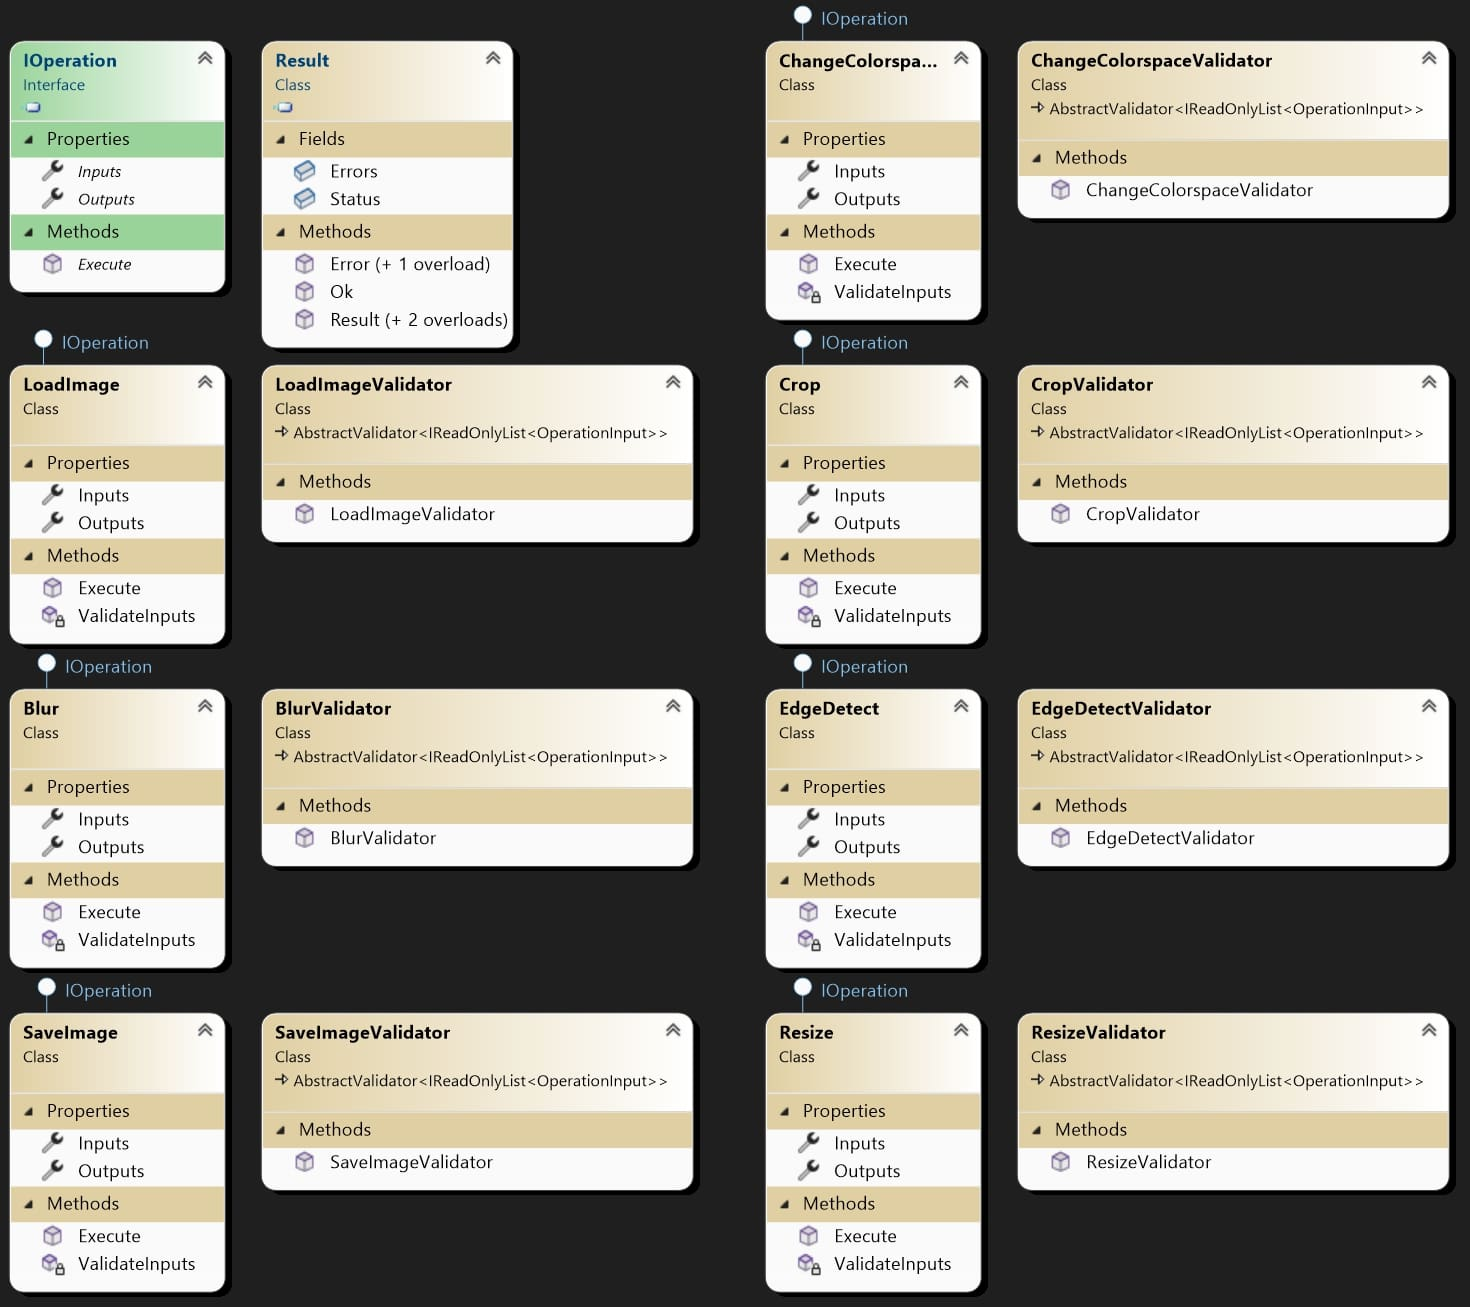
\includegraphics[width=1\linewidth]{images/Picture11.jpg}
    \caption{Diagram operacji. Opracowanie własne.}
    \label{fig:modelDiag}
\end{figure}

W NoodleCV warstwa \textit{Model} jest minimalna \autoref{fig:modelDiag}. 
Posiada interfejs IOperation odpowiadający za formę wszystkich implementacji operacji. 
Posiadają generyczna kolekcje wejść \textit{Inputs} oraz wyjść \textit{Outputs}.
Jedyna metoda zdefiniowana w nich to wykonanie operacji - zwraca ona obiekt \textit{Result}.
Informuje ona następne warstwy czy operacja się powiodła, jeżeli nie to dodatkowo zawiera listę błędów. 
Walidację wykonujemy sprawdzając wejścia za pomocą biblioteki Fluent Validation. 
Każda operacja wymaga swojego własnego walidatora danych i zapewnia tym bezpieczne działanie aplikacji - użytkownik nie powinien być w stanie doprowadzić programu do błędu złym parametrem operacji.

\begin{figure}[H]
    \centering
    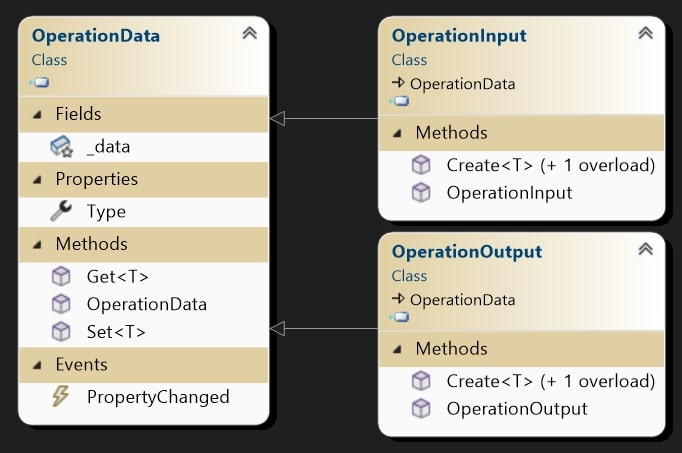
\includegraphics[width=0.6\linewidth]{images/Picture12.jpg}
    \caption{Diagram generycznych typów przechowujących dane operacji. Opracowanie własne.}
    \label{fig:input}
\end{figure}

Wejścia i wyjścia parametrów operacji mogą być w wielu różnych typach więc kolekcje przyjmujące te dane musiały być generyczne. 
Daje to dużo większą elastyczność, ale może utrudnić implementację. 
Tworząc operacje i ich późniejsze \textit{ViewModel}'e trzeba zachować szczególną ostrożność. 
Przy tworzeniu nowych modeli zakładamy że obiekt w tym miejscu kolekcji będzie miał odpowiedni typ. 
Przy odczytywaniu danych z tej kolekcji nie ma informacji co to za klasa, należy poprawnie narzucić jej rodzaj inaczej napotkamy błąd i aplikacja wyłącza się.
Pomimo tych problemów warto korzystać z tej struktury ponieważ niektóre operacje przyjmują tylko ścieżkę do pliku w formie tekstu, inne mogą nie mieć żadnego wyjścia ale wszystkie pasują do jednego wspólnego interfejsu.

\subsubsection{View} 

\begin{figure}[H]
    \centering
    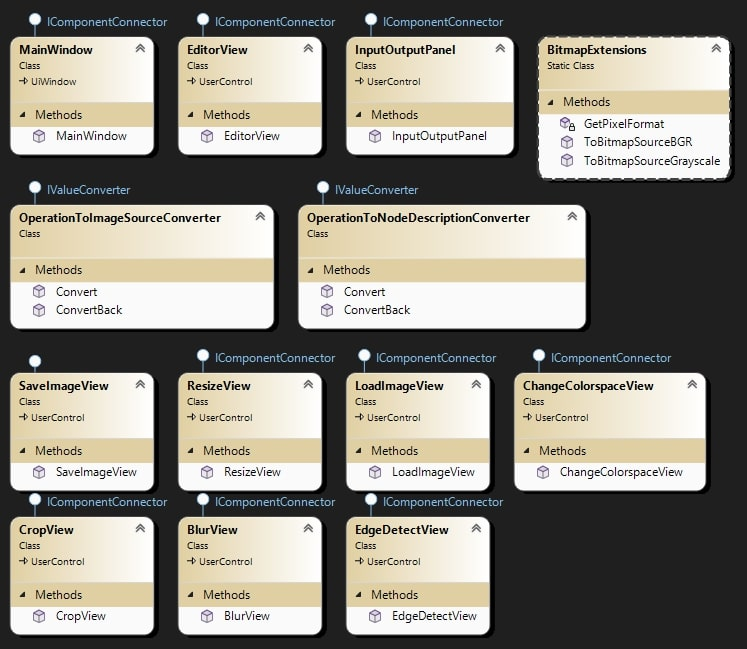
\includegraphics[width=0.8\linewidth]{images/Picture19.jpg}
    \caption{Diagram klas używanych do tworzenia interfejsu. Opracowanie własne.}
    \label{fig:viewArch}
\end{figure}

Warstwa widoku składa się z głównego okna, edytora i jego elementów.
Dodatkowo użyto klasy statycznej posiadającej metody pozwalające na konwersję obrazów z formatu używanego przez operacje na format akceptowany przez wyświetlanie obrazu w WPF.
Drugi konwerter zajmuje się pobieraniem danych z obrazu przetwarzanego przez operację i stworzenie opisu zawierający jego rozmiar oraz ilość kanałów koloru.

\begin{figure}[H]
    \centering
    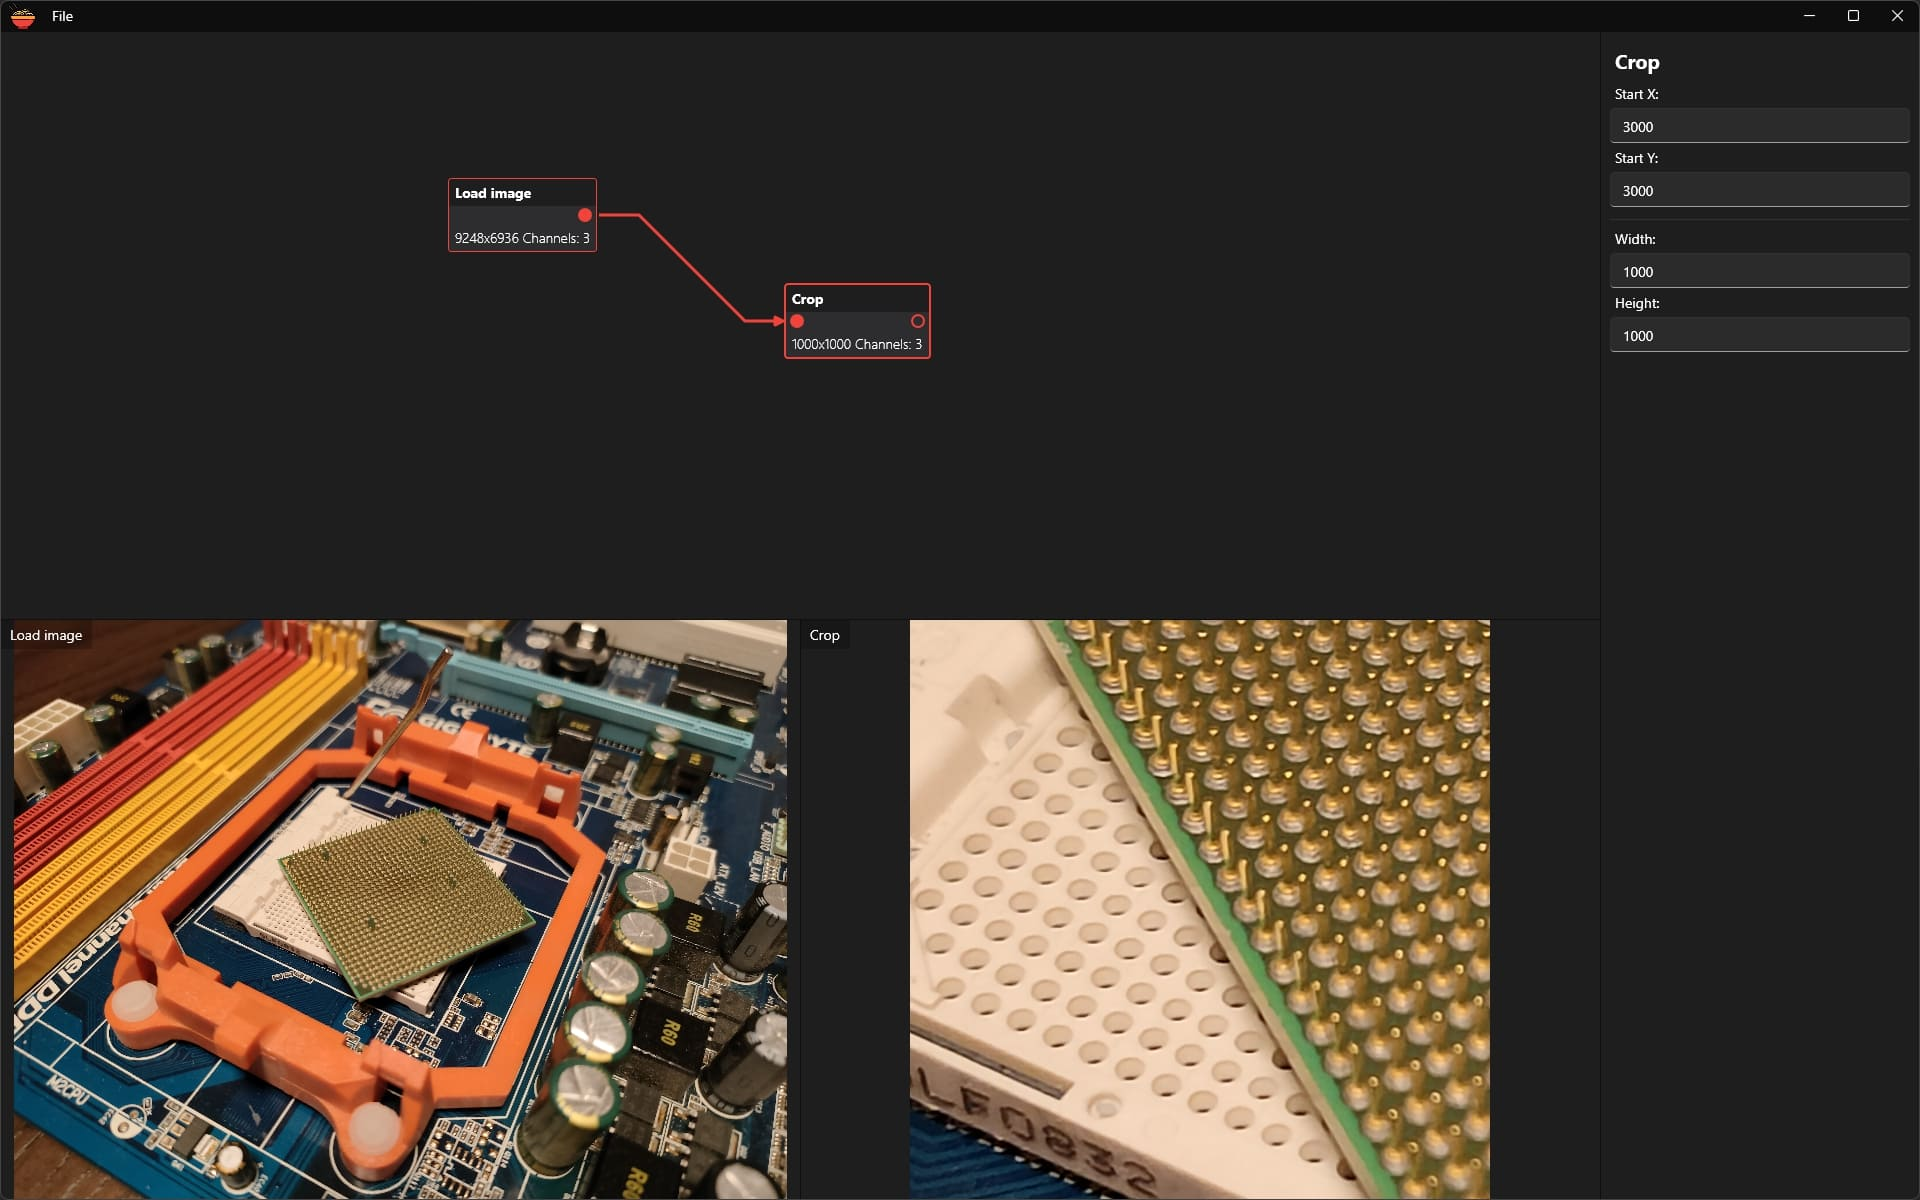
\includegraphics[width=1\linewidth]{images/Picture13.jpg}
    \caption{Główne okno aplikacji z przykładowymi operacjami. Opracowanie własne.}
    \label{fig:window}
\end{figure}

Aplikacja posiada jedno okno \autoref{fig:window}. 
Użyta została klasa \textit{UiWindow} z biblioteki WPF UI \cite{wpfui} pozwalająca łatwo zmodyfikować górny pasek by pasował do nowoczesnych systemów operacyjnych. 

\begin{figure}[H]
    \centering
    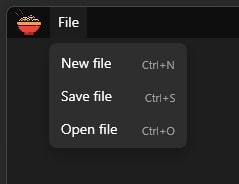
\includegraphics[width=0.6\linewidth]{images/Picture14.jpg}
    \caption{Menu aplikacji. Opracowanie własne.}
    \label{fig:mainmenu}
\end{figure}

Menu pozwala na zapisywanie odczytywanie lub czyszczenie stanu aplikacji. 
Opcje te są też przypisane znanym skrótom klawiszowym w celu ułatwienia ich używania.

Zawartość okna znajduje się w osobnym widoku edytora. Jest on podzielony na 3 główne elementy. Edytor (\autoref{fig:editor}) gdzie dodaje się nowe operacje, podgląd (\autoref{fig:preview}) gdzie pojawiają się wyniki operacji i panel od modyfikacji parametru (\autoref{fig:params}).

\begin{figure}[H]
    \centering
    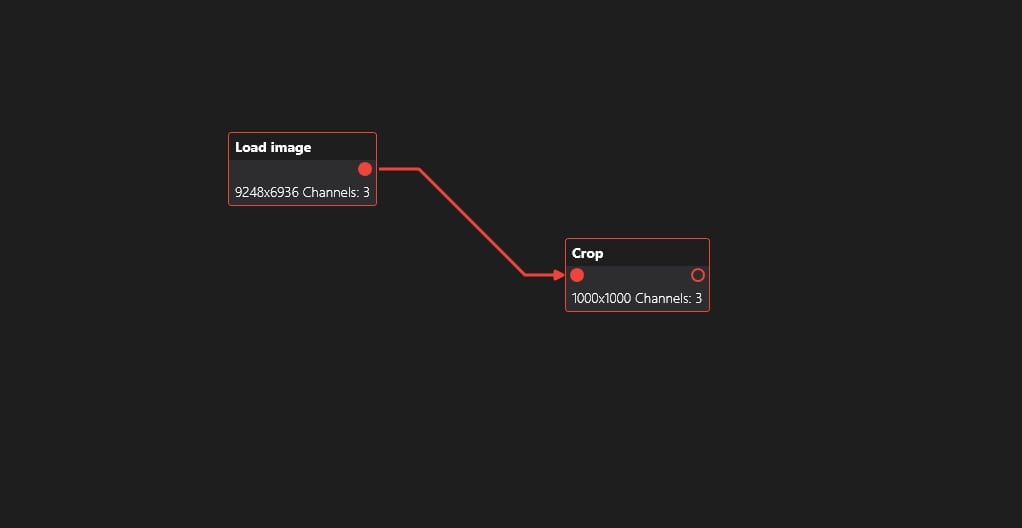
\includegraphics[width=1\linewidth]{images/Picture15.jpg}
    \caption{Widok edytora. Opracowanie własne.}
    \label{fig:editor}
\end{figure}

W tej części widoku użytkownik może dodawać nowe operacje, łączyć je, przeciągać oraz wybierać i zmieniać parametry wybranych bloczków. 
Operacje dodajemy za pomocą menu kontekstowego (\autoref{fig:context}) umieszczonego w edytorze. 
Otwiera się je za pomocą kliknięcia prawego przycisku myszy na jego obszarze.
Węzły stworzone w ten sposób posiadają nagłówek odpowiadający nazwie operacji którą reprezentują oraz połączenia wejściowe i wyjściowe reprezentujące możliwe połączenia.
Po uzyskaniu rezultatu pojawia się też informacja jakiego rozmiaru jest obraz znajdujący się na wyjściu i ile kanałów posiada - czy to obraz biało-czarny lub kolorowy.
Są to elementy biblioteki Nodify \cite{nodify} ze zmodyfikowanymi stylami w celu utrzymania jednolitej stylistyki projektu.

\begin{figure}[H]
    \centering
    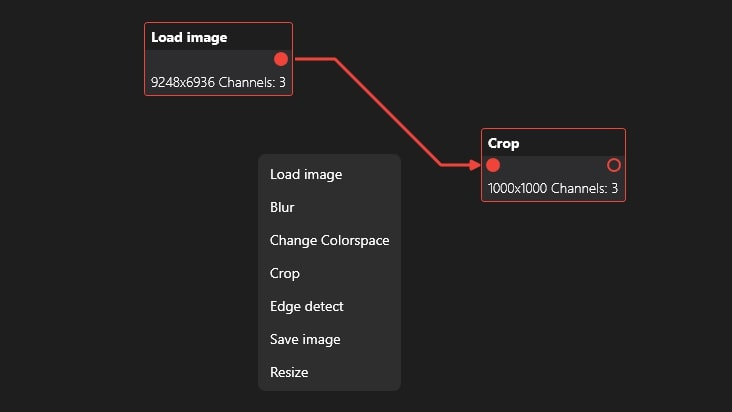
\includegraphics[width=0.6\linewidth]{images/Picture18.jpg}
    \caption{Menu kontekstowe edytora. Opracowanie własne.}
    \label{fig:context}
\end{figure}


Po dodaniu operacji zostaje ona automatycznie przypisana do podglądu obrazu (\autoref{fig:preview}) umieszczonego pod edytorem. Użytkownik może później zmienić i wybrać które elementy są wyświetlane za pomocą klawiszy `1' i `2'.

\begin{figure}[H]
    \centering
    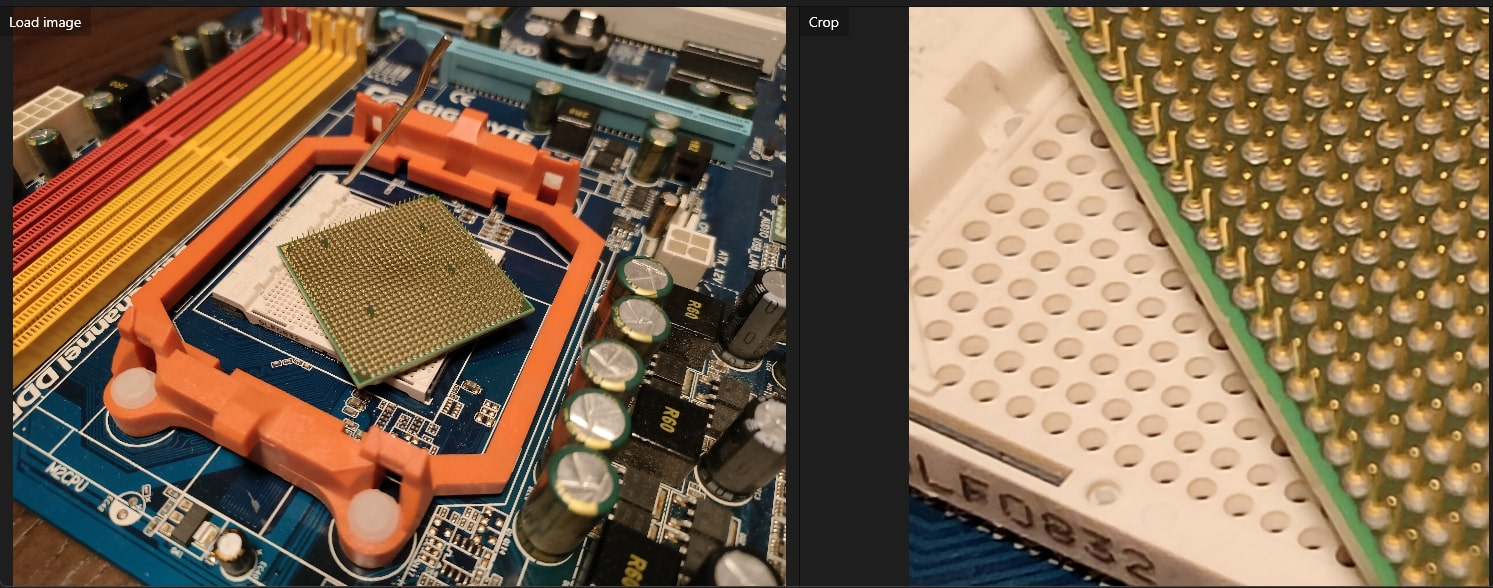
\includegraphics[width=1\linewidth]{images/Picture16.jpg}
    \caption{Podgląd wyników operacji. Opracowanie własne.}
    \label{fig:preview}
\end{figure}

\begin{figure}[H]
    \centering
    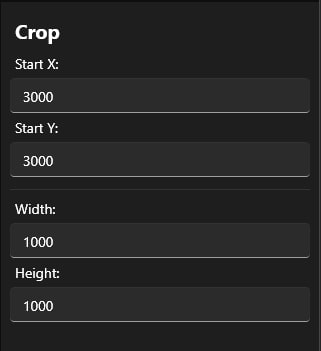
\includegraphics[width=0.6\linewidth]{images/Picture17.jpg}
    \caption{Edycja parametrów. Opracowanie własne.}
    \label{fig:params}
\end{figure}

Ostatni element widoku aplikacji to panel (\autoref{fig:params}) gdzie można edytować parametry wybranej operacji. 
Każdy węzeł potrzebuje swojego osobnego widoku który poprawnie odwzorowuje parametry potrzebne do wykonania operacji. 
Są one przypisane do pól w odpowiednich ViewModeli i każda zmiana użytkownika jest przesyłana do niego w celu zaktualizowania wyników operacji.

\begin{figure}[H]
    \centering
    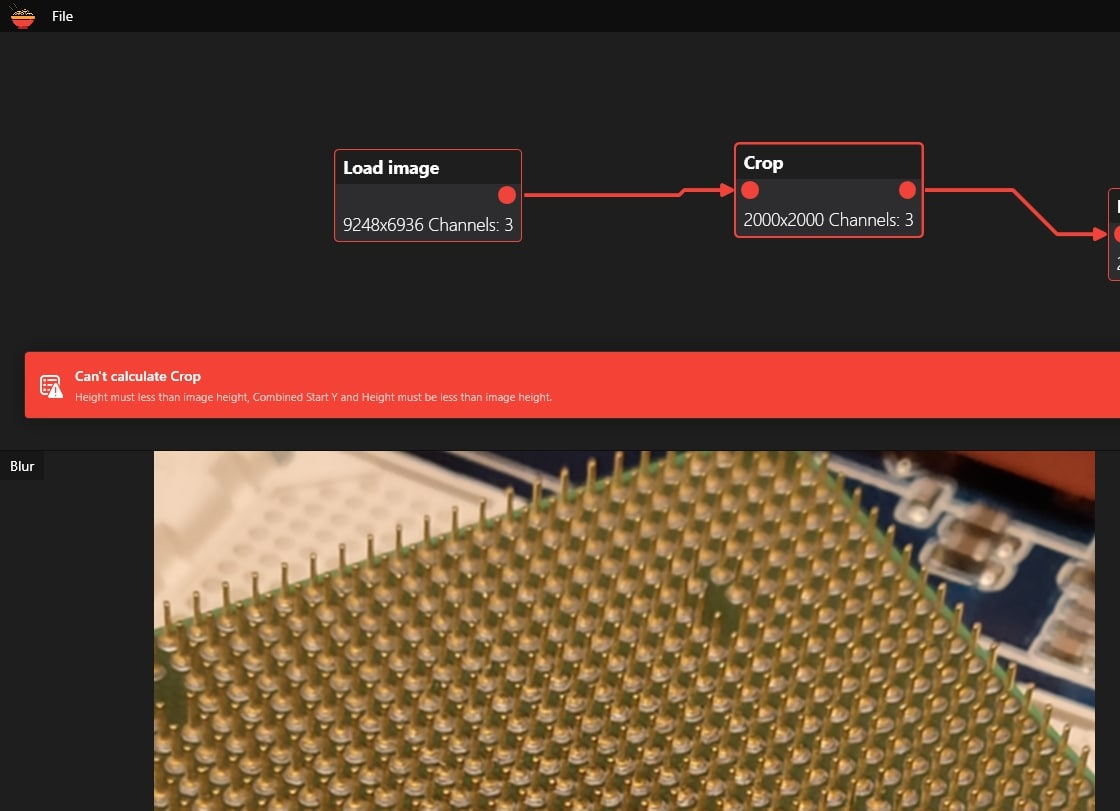
\includegraphics[width=0.8\linewidth]{images/Picture31.jpg}
    \caption{Komunikat z błędem. Opracowanie własne.}
    \label{fig:error}
\end{figure}

Po wprowadzeniu nieprawidłowej wartości pojawia się czerwony komunikat (\autoref{fig:error}) wskazujący dlaczego operacja nie mogła się wykonać.

\subsubsection{ViewModel}

W przypadku tego projektu warstwa komunikacji między modelem i widokiem jest najbardziej obszerna. 
Większość z tych klas dziedziczy po ViewModelBase wziętym z \textit{BindableBase} \cite{prismlibraryprism} z biblioteki \textit{Prism} \cite{prismlibrary}. 
Znajdują się w nim metody pomagające z obsługą interfejsu IPropertyChanged. 
Jest on kluczowy w tworzeniu aplikacji reagującej natychmiastowo na dane wejściowe od użytkownika w technologii WPF. 
Dają one znać komponentom do których przypisane są wartości, że się zmieniły i trzeba je zaktualizować.


\begin{figure}[H]
    \centering
    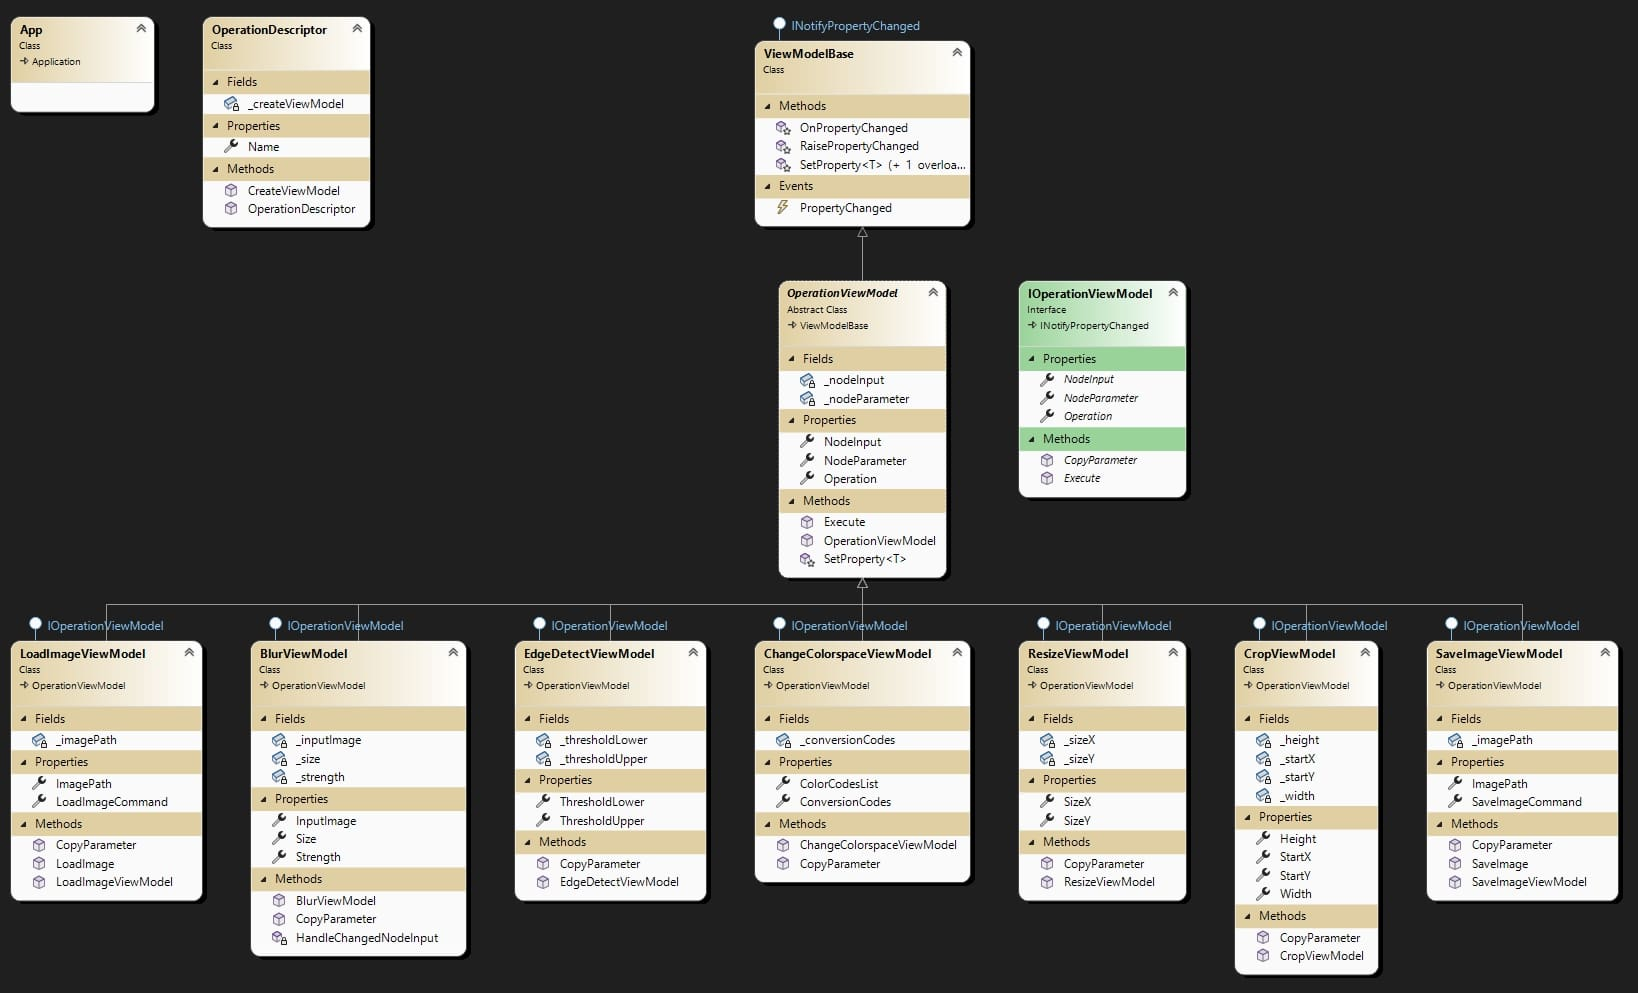
\includegraphics[width=1\linewidth]{images/Picture20.jpg}
    \caption{Diagram ViewModeli operacji. Opracowanie własne.}
    \label{fig:vmDiagOperation}
\end{figure}

Każda operacja potrzebuje swój ViewModel. Dbają one o poprawne wyświetlanie i przypisanie wartości z modelu. Zajmują się też uruchomieniem obliczeń i zwróceniem ich rezultatu. Każdy z nich posiada też metodę pozwalającą na skopiowanie parametrów z innej operacji. Jest to wykorzystane przy odczytywaniu danych z zapisanego stanu.

\begin{figure}[H]
    \centering
    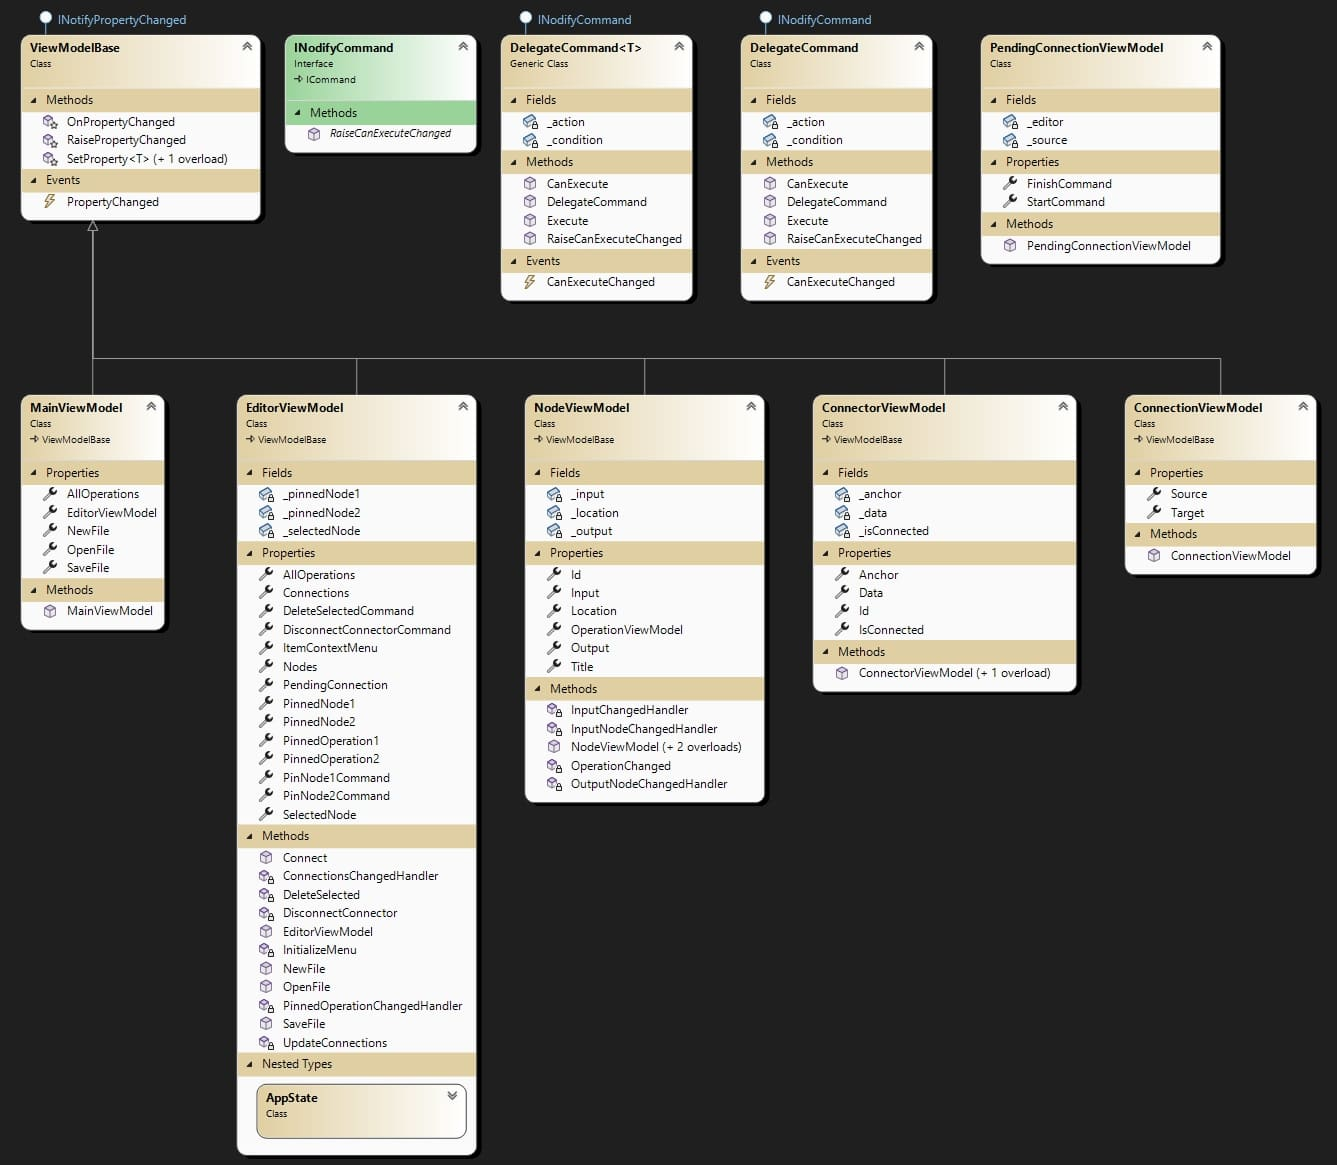
\includegraphics[width=1\linewidth]{images/Picture21.jpg}
    \caption{Diagram ViewModeli aplikacji. Opracowanie własne.}
    \label{fig:vmDiagEditor}
\end{figure}

Pozostałe ViewModele dalej korzystają z tej samej klasy bazowej.
MainViewModel tworzy jedynie komendy do których odnosi się menu główne, większość logiki programu jest umieszczona w EditorViewModelu.
Jest tam umieszczona kolekcja przechowująca stworzone węzły i ich stany oraz połączenia między nimi.
Klasa NodeViewModel odpowiada bloczkom w edytorze. Przechowują one ViewModel odpowiedniej operacji, ale też pozycje na ekranie wraz z wejściami i wyjściami. 
Są to obiekty typu ConnectorViewModel między którymi tworzą się połączenia przesyłające dane między węzłami. 
